\documentclass[11pt,titlepage]{article} % use larger type; default would be 10pt
\usepackage{mathrsfs,amsmath}
\usepackage{gensymb}
\usepackage{graphicx}
\usepackage{cite}
\usepackage{indentfirst}
\usepackage{float}
\usepackage[hidelinks]{hyperref}
%\usepackage{floatrow}%
\graphicspath{ {images/} }
\usepackage{fixltx2e} %for subscript
\usepackage[margin=0.6in]{geometry}
\setlength{\parskip}{\baselineskip}%
\setlength{\voffset}{0in}
%\bibliographystyle{ieeetr}  
\linespread{1.5}
%\pagenumbering{gobble}

\title{Literature Review: Ultrasound, Microbubbles, and the Blood-Spinal Cord Barrier}
\author{Rui Xu\\MBP Rotation 1}
\date{} % Activate to display a given date or no date (if empty),
         % otherwise the current date is printed 
         
\begin{document}
\maketitle

%\tableofcontents
\newpage


\section{Introduction}

This project aims to use focused ultrasound and microbubbles to open the human Blood-Spinal Cord Barrier (BSCB). This project will build on previous work that used ultrasound and microbubbles to open the Blood Brain Barrier (BBB) in humans, as well as previous BSCB work in animal models. The primary goal of the first rotation is to build a simulation for ultrasound propagation to the spinal cord to optimize the design of an ultrasound transducer specific to this BSCB application. 

\section{Anatomy and Physiology of the Spine}

To begin, we discuss the various aspects of the spine that will be important for this project. There are two main components of the spine that we will consider - the vertebral column and the spinal cord.

\subsection{The Vertebral Column}
The spine vertebral is composed of irregular bones called vertebrae. Each vertebrae has a body, a centrum, and a vertebral (neural) arch. The body is composed of cancellous (trabecular) bone, and covered in cortical (compact) bone. Bone generally consists of bone matrix, which is approximatepy 35$\%$ organic and $65\%$ inorganic material, by weight. Organic material is primarily collagen and proteoglycans. The inorganic material consists primarily of hydroxyapatite (Ca$_{10}$(PO$_4$)$_6($OH$)_2$. Bone tisse is classified as either woven or cancellous, otherwise known as lamellar. Lamellar bone is mature bone organized into lamellae approximately 3-7$\mu$m thick. Bone can also be classified by the volume fraction of the bone. Spongy bone consists of interconnecting rods and plates called trabeculae, and the space between the trabeculae is filled with blood vessels and bone marrow in living organisms. Compact bone has more bone matrix than spongy bone \cite{vanputte2016seeley}. 

There are thirty three vertebrae in the vertebral column - seven cervical, twelve thoracic, five lumbar, and five fused sacral vertebra. Each vertebra has a spinous process on the posterior side, transverse processes on the lateral sides, and various facets for interactions with neighbouring vertebrae and ribs in the case of thoracic vertebra. An annotated diagram of a vertebra is shown in Figure \ref{vertebra}.
\begin{figure}[H]\label{vertebra}
\centering
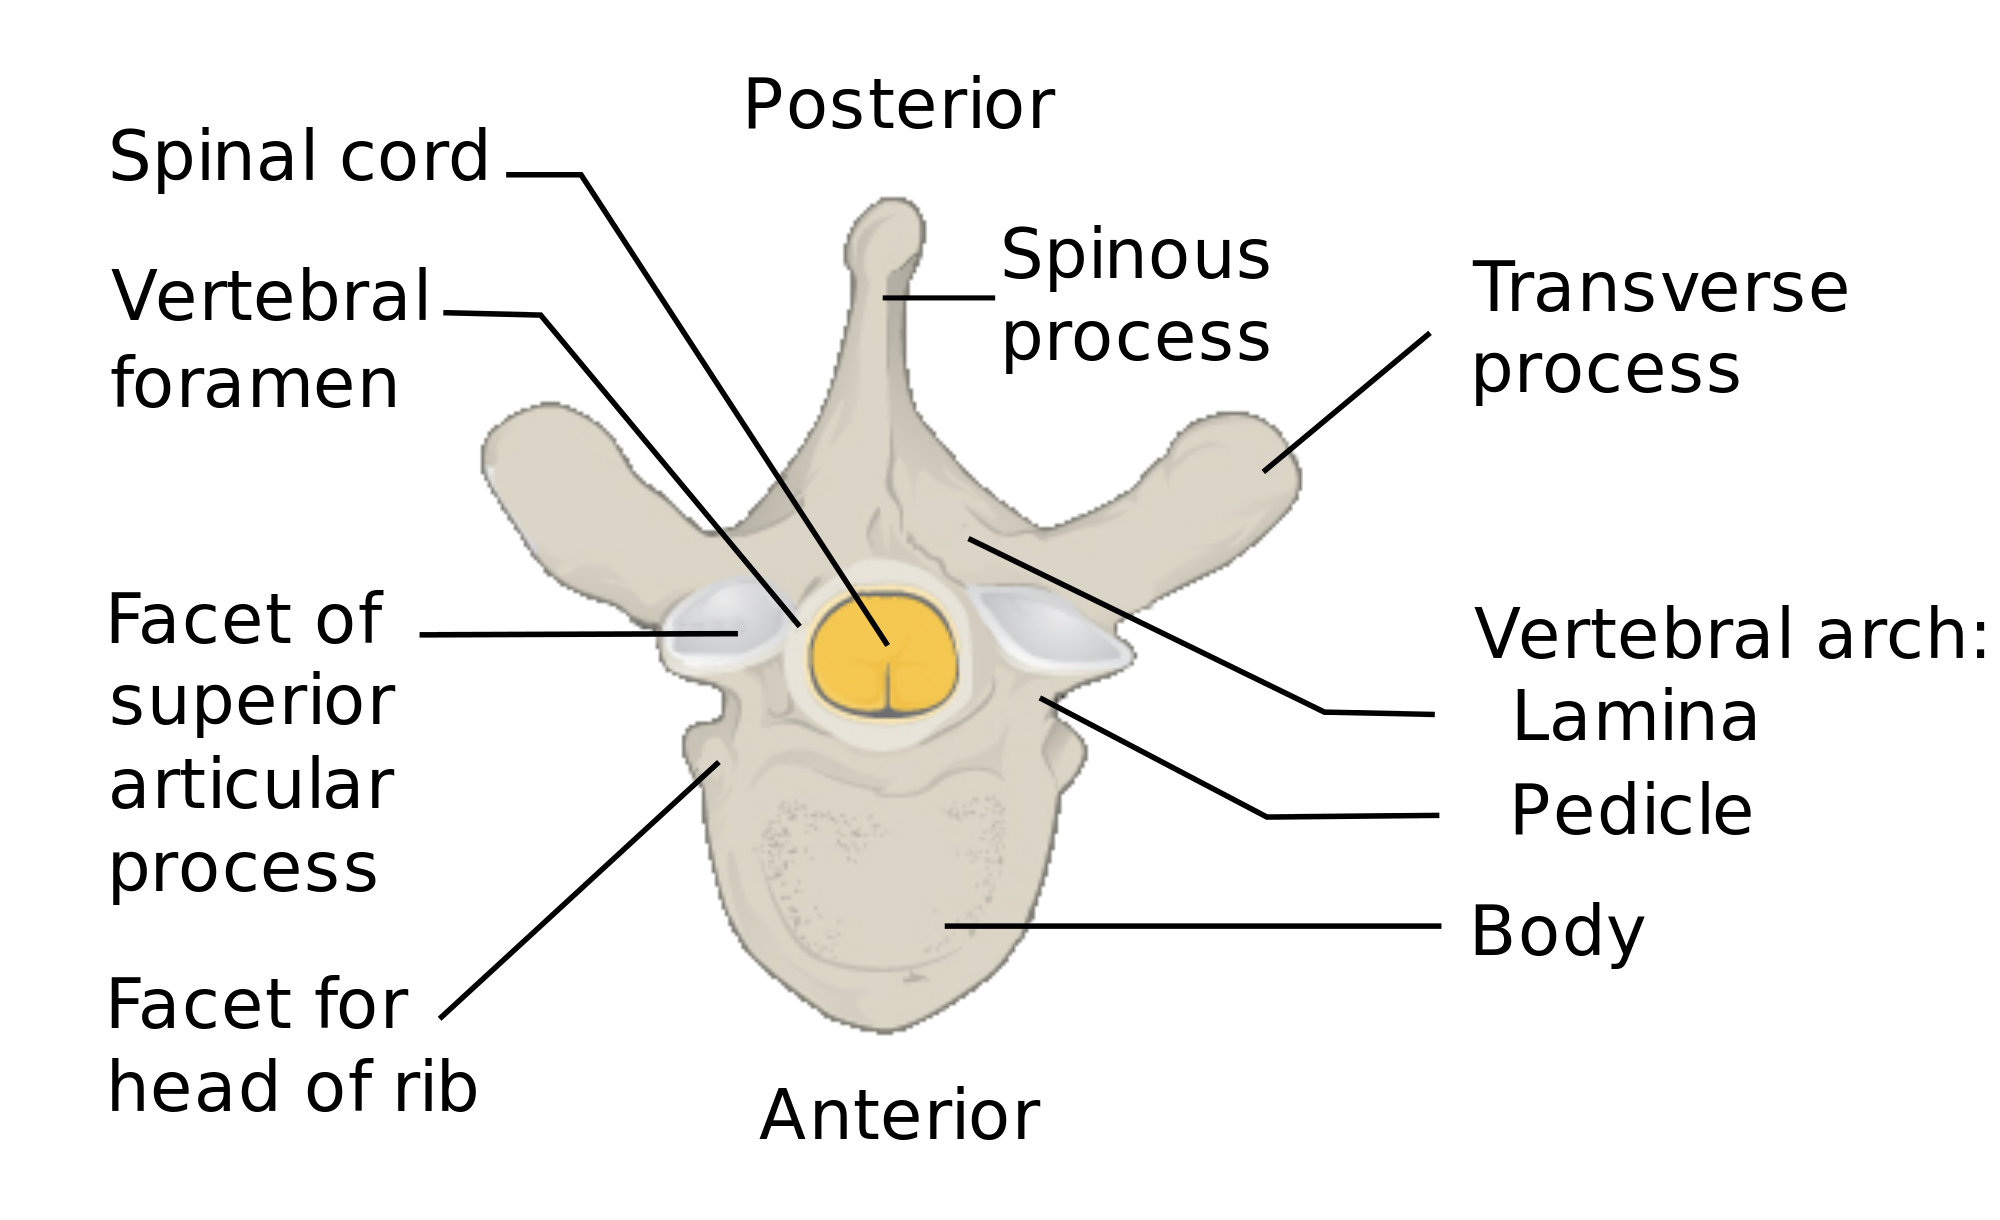
\includegraphics[scale=0.25]{vertebrae}
\caption{An annotated diagram of a thoracic vertebra, from \href{https://commons.wikimedia.org/wiki/File:Vertebra_Superior_View-en.svg}{Wikimedia Commons}.} 
\end{figure}

The body of the vertebra is roughly disk shaped, and usually the largest part with superior and inferior flat surfaces. The body forms the anterior wall of the vertebral foramen, and vertebral disks are located between the bodies of two vertebrae. The vertebral foramen is the hole in each vertebra through which the spinal cord passes, and the vertebral canal is composed of adjacent vertebral foramen. The vertebral arch forms the lateral and posterior walls of the vertebral foramen, and is decorated with spinous, articular, and transverse processes, as well as multiple articular surfaces. The anatomy of the vertebral arch is further broken down into the pedicle, lamina, and various processes. THe pedicle is the foot of the vertebral arch, with one on each side of the arch. The lamina is the posterior part of the arch, which forms the posterior wall of the vertebral foramen. The transverse processes projects laterally from the junction of the pedicle and lamina, and are sites for muscle attachment. The spinous process projects posteriorly from the junction of the two lamina, is a site for muscle attachment, and also strengthens the vertebral column and allows for movement. Each vertebrae has inferior and superior processes with facets where vertebrae articulate with one another. There are also intervertebral notches, which form intervertebral foramina between two adjacent vertebrae for spinal nerves to exit the vertebral foramen.


\subsection{The Spinal Cord}
The central nervous system is composed of the brain and the spinal cord. The spinal cord serves as a conduit for motor control output and sensory input, as well as a central processing centre for certain reflexes. Similarly to the brain`s BBB, the spinal cord has a BSCB. The BBB and BSCB are constructed of the same morphological building blocks, but physiological differences between the two mean that the BSCB is considered a separate entity \cite{bartanusz2011blood}

Similarly to the BBB, the BSCB is constructed from nonfenestrated endothelial cells linked with tight junctions, and their accessory structures (basement membrane, pericytes, astrocytic end feet processes). However, the BSCB has glycogen deposits in the microvessels of the spinal cord, and the BSCB has slighly increased permeability for certain molecules such as interferons \cite{sharma2005pathophysiology,pan1997permeability}. However, the BSCB much like the BBB is a barrier to drug development as most drugs targeting the spinal cord must be injected locally and through the intrathecal route, which is highly invasive. Therefore it is highly desireable to disrupt the BSCB, temporarily increasing its permeability such that large molecules may cross the BSCB. One such method involves the use of focused ultrasound and microbubbles. This method has been implemented successfully in opening the BBB and the BSCB. For example, focused ultrasound and microbubbles have been implemented in mouse models, allowing the passage of molecules such as genes across the BSCB for the treatment of spinal injury and disease \cite{weber2015gene}. We hope to extend this method to the human BSCB, and part of this extension requires the design of an ultrasound transducer that will deliver the appropriate ultrasound exposure/dose to the spinal cord, without excess energy deposition and heating at the various irregular interfaces between the vertebrae, soft tissue, and the spinal cord. 


\section{Ultrasound and the Spine}

In this section I'll discuss current research with Ultrasound and the Spine. As mentioned in the previous section, magnetic resonance guided focused ultrasound (MRI-g-FUS) has been used to open the BSCB in mouse models to mediate gene delivery administered intravenously\cite{weber2015gene}. Ultrasound can be scattered and absorbed by heterogeneous bone structures, which adds complexity to FUS application around the highly irregular vertebrae. Building a task specific ultrasound transducer requires good understanding of the possible interactions between ultrasound waves and the vertebrae. There are two main avenues for investigating these interactions - experiment and computation. 

\subsection{Experimental Results}

\textbf{Notes from 'Feasibility of Transient Image-guided Blood-Spinal Cord Barrier Disruption' \cite{wachsmuth2009feasibility}.}\\
Rats were exposed to focused 1.08MHz ultrasound, power 0.5 and 1.0W, used ultrasound contrast agent 'Definity'. The Definity contrast agent is composed of lipid-coated microspheres filled with octafluoropropane gas, have a mean diameter of 1.1 to 3.3 $\mu$m, and are stable enough to pass through pulmonary capillaries. The microbubbles have lower aoustic impedance than blood. \\
Transducer: 1.08MHz, 7cm diameter, f-number = focal length / diameter = 0.8, so focal length was 0.8*7 = 5.6cm. Bolus of ultrasound microbubbles (what is this, exactly?) administered before sonication. Measurement of BSCB opening is through signal enhancement, and demonstrated in paper as `relative enhancement' over the baseline value, and were determined to be 29.1 $\pm 21\%$ and $57.5 \pm 34\%$ at 0.5 and 1.0 watts respectively. Article concludes discussion section with 'The propagation of the acoustic wave is certainly affected by the presence of this bone (bony vertebrae), and so strategies to compensate for this effect are required.\\


\textbf{Notes from Longitudinal and shear mode ultrasound propagation in human skull bone \cite{white2006longitudinal}.}
For years it was thought that energy propagation through bone was primarily through the longitudinal mode, with minimal energy propagation through the shear modes. However, mode conversion from fluid to shear modes in elastic media such as the skull can be efficient, as the speed of sound in fluids is closely matched by the shear speed of sound in elastic media like the bone. For example, in \cite{white2006longitudinal}, the shear speed of sound for a 1.0MHz source was measured to be 1500m/s, and was found to transmit up to 36$\%$ of the longitudinal pressure amplitude.  


\textbf{Notes from `The dependenc of ultrasonic properties on orientation in human vertebral bone' \cite{nicholson1994dependence}.}
The authors made measurements of the speed of sound and broad-band ultrasound attenuation in cubes of human trabecular bone from lumbar vertebrae along the cranio-caudal (CC) axis, the lateral (LT) axis, and the antero-posterior (AP) axis.
The authors found that $\nu_s$ was appproximately 500m/s greater along the CC axis than the LT and AP axes. The authors also found that the broad-band ultrasound attenuation was approximately 23dB/MHz/cm greater for the CC axis. The authors suggest that the anomalous CC axis results are due to a transient (transient what?) travelling ahead of the main wavefront, suggesting that ultrasound propagates directly through the trabecular framework as a bar wave, allowed by the  trabecular structure which is primarily oriented along the direction of ultrasound propagation. This makes sense because vertebrae are primarly loaded in the vertical direction. The frequency rage used in this study was 0.2-0.6MHz. Results for speed of sound:

\begin{table}[!h]
\begin{center}
  \begin{tabular}{| c | c | c | c | c | }
    \hline
     & Mean & SD & Max & Min \\ \hline
     CC & 1918 & 305 & 2469 & 1506 \\ 
     AP & 1761 & 119 & 2027 & 1599 \\ 
     LT & 1709 & 114 & 2065 & 1575 \\ 
     CCm & 2249 & 124 & 2534 & 2024 \\
    \hline
  \end{tabular}
\end{center}
\caption{Speed of sound along various axes. CCm means modified results along the cranio-caudal axis, obtained by increasing the gain of the digitizer in order to repeatably be able to observe the transident preceding the main wave}
\end{table}
 
 Results for broad-band ultrasound attenuation:
 \begin{table}[!h]
\begin{center}
  \begin{tabular}{| c | c | c | c | c | }
    \hline
     & Mean & SD & Max & Min \\ \hline
     CC & 15.0 & 20.6 & 79.5 & 1.3 \\ 
     AP & 12.4 & 7.5 & 37.1 & 5.0 \\ 
     LT & 10.5 & 6.9 & 37.6 & 4.1 \\ 
     CCm & 34.0 & 22.4 & 79.9 & 11.9 \\
    \hline
  \end{tabular}
\end{center}
\caption{Broad-band ultrasound attenuation along various axes. CCm means modified results along the cranio-caudal axis, obtained by increasing the gain of the digitizer in order to repeat-ably be able to observe the transident preceding the main wave}
\end{table}

Density is independent of orientation, so in order to accurately model would we need some sort of ultrasound propagation tensor for each point? 

\textbf{Notes from Acoustic properties of the human skull \cite{ fry1978acoustical}}.
Phase speeds for `ivory tables' measured to be 2960m/s in skull bone.

\textbf{Notes from Physical Properties of Tissues \cite{duck1990physical}}
I searched `vertebra' in the handbook. Density between 1300-1420kg/m$^3$ for vertebral bone. US velocity in spinal cord is 1542m/s. Trabecular bone density 1080kg/m$^3$. Cortical bone density 1990kg/m$^3$. Trabecular bone 1688-2084m/s. Really wide range of values. Cortical bone 3526m/s in femur, some measurements up to 4000m/s.


\subsection{Computational Results}

\textbf{Notes from Interstitial ultrasound ablation of vertebral and paraspinal tumours: Parametric and patient-specific simulations \cite{scott2014interstitial}.}\\
This work investigates the theoretical and patient specific feasibility of treating tumours using thermal ultrasound.
They used 3D patient specific models, and simulated various applicator configurations, frequencies (high frequency 3 and 7MHz, not trying to penetrate/traverse bony structures), placement trajectories (? not sure what this is), and gaseous insulation.\\
Bone has a high acoustic absorption coefficient ($\alpha_0$) relative to soft tissue, generally between one and two orders of magnitude higher \cite{duck1990physical}. This causes heating at the interface of the bone with the soft tissue, and prevents ultrasound penentration into the bony structure \cite{fujii1999study}. <- read paper in more detail\\
The interstitial US applicators were modelled as a linear array of 1-4 tubular ultrasound transducers, with 150 to 360 degree angular sectors(need to look up what this means exactly?)\\
The main goal of this work was the evaluate thermal energy deposition, so they implement the Pennes' Bioheat transfer equation for heterogeneous tissues \cite{pennes1948analysis}:
\begin{equation}
\rho c \frac{dT}{dt} = \nabla \cdot k \nabla - \omega c_b(T-T_b)+Q
\end{equation}
where $\rho$ is density (kg/m$^3$), $c$ is specific heat capacity (J/kg/$^{\circ}$C), $T$ is temperature ($^{\circ}$C), $k$ is thermal conductivity (W/m/$^{\circ}$C), $\omega$ is blood perfusion (kg/m$^3$/s), $c_b$ is the specific heat capacity of blood, $T_b$ is the temperature of blood, and $Q$ is heat energy deposited by the ultrasound source. \\
This paper also describes the method they use to calculate thermal dose, according to the method devised by \cite{sapareto1984thermal}, as well as a method for calculating $Q$ based on radial distance from the applicator, the transmission coefficient of the tissue (read \cite{scott2013interstitial} as well).\\
Generation of patient specific done by segmentation of CT image, surface reconstruction, FEM mesh generation, Temperature map.\\
See table 1 for material properties. Many of them are cited from \cite{duck1990physical}.
There is little mention of the computer simulation in this paper, except that it uses COSMOL and Matlab\\


\textbf{Notes from Three-dimensional simulation of ultrasound propagation through trabecular bone structures measured by synchrotron microtomography \cite{bossy2005three}.}
Simulation of ultrasound propagation through trabecular bone samples measured using synchotron microtomography, which gives high resolution mapping of the bone structures.
Used in house simulation software called 'simsonic', a finite-difference time domain algorithm often used in geophysics.This algorithm is used because it is good for both solids and fluids \cite{graves1996simulating}\\
Cancellous (trabecular) bone is anisotropic, heterogeneous, and has two phases - interconnected plates/rods that are immersed in marrow. \\
Properties include: attenuation varies linearly with frequency (three citations available here), sound velocity and frequency-attenuation relationship are highly correlated with bone volume fraction (porosity), velocity dispersion generally negative but occasionally positive, 2 compressional waves can propagate along a direction of a trabecular network (what does this mean?)\\
Bone samples from femurs, defatted, image pixels 10$\mu$m turned into a binary map for the simulation. Segmentation threshold " between two well separated pixel distributions corresponding to bone and air pores. Tissue properties for simulation: $\rho = 1.85$g/cm$^3$, compressional bulk velocity = 4000m/s, shear wave velocity = 1500m/s.\\


\textbf{Notes from `The finite element method for micro-scale modeling of ultrasound propagation in cancellous bone' \cite{vafaeian2014finite}. }
The finite-difference time-domain method has two disadvantages for modelling ultrasound propagation in bone. The first is staircase sampleing of cancellous bone by finite difference grids, which leads to wave artefacts at the solid-fluid interface within the bone. The second disadvantage is it can't satisfy the perfect-slip condition at the interface, a condition that occurs at a solid-fluid interface if there is no interfacial friction. 
Methods and frameworks for US propagation in bone include: Biot's theory, stratified or multilayer models, scattering model, and microscale models. 
Micro-scale models - based on virtual geometries of trabecular networks spatially sampled and served as discrete domains for numerical simulations. The geometry is generated from $\mu$-CT images or imitations. This method has had relatively good success. 

\textbf{Notes from `The Contribution of Shear Wave Absorption to Ultrasound Heating in Bones: Coupled Elastic and Thermal Modeling' \cite{treeby2015contribution}.}
In this paper, by the creators of k-wave, the authors investigate the heating of bone by ultrasound using a coupled elastic wave model and bioheat transfer equation. The volume rate of heat deposition by compressional waves and shear waves are calculated separately by splitting acoustic particle velocity using a `k-space diadic'. At normal incidence, then heating is dominated by the absorption of compressional waves. At angles of incidence greater than ten degrees, then shear wave contribution becomes significant.
Used four long-bone geometries in the experiment - 1. half space 2. solid bone layer 3. hollow bone layer, containing marrow 4. anthropomorphic bone layer derived from a segmented CT scan, also containing marrow. Sonication angles were from 0$^{\circ}$ to 60$^{\circ}$. The material properties the authors used are included in the following table. 
 \begin{table}[!h]
\begin{center}
  \begin{tabular}{| c | c | c | c | c | }
    \hline
     & Soft Tisse & Bone & Marrow & Units \\ \hline
     density $\rho_0$ & 1090 & 1900 & 928 & kg/m$^3$ \\ 
     sound speed compression $c_P$ & 1580 & 2820 & 1430 & m/s \\ 
     sound speed shear $c_S$ & N/A & 1500 & N/A & m/s \\ 
     absorption compression $\alpha_P$ & 0.57 & 9 & 0.6 & dB/(MHz$^2$cm) \\
     absorption shear $\alpha_S$ & N/A & 20 & N/A & dB/(MHz$^2$cm) \\
	 specific heat & 3400 & 1300 & 2740 & J/(kg.K)\\
	 thermal conductivity & 0.5 & 0.3 & 0.22 & W/(m.K)\\
    \hline
  \end{tabular}
\end{center}
\caption{Acoustic properties of tissues used in \cite{treeby2015contribution}, originally from \cite{duck1990physical}}
\end{table}
\linespread{1.0}
The authors calculated volume rate of heat deposition $Q$ using the steady state particle velocity amplitude \textbf{u}, where the heat deposition due to compressional waves $Q_P$ is given by:
\begin{equation}
Q_P = \alpha_P \rho_0 c_P u_P^2
\end{equation}
and the heat deposition due to shear waves $Q_S$ is given by:
\begin{equation}
Q_P = \alpha_S \rho_0 c_S u_S^2
\end{equation}
where the $S$ and $P$ subscripts denote shear and compressional waves respectively, $\alpha$ denotes the absorption coefficients, $\rho_0$ is density, $c$ is the speed of sound, and $u^s$ is $\textbf{u} \cdot \textbf{u}$. The method for separating the compressional and shear components of the particle velocity are described in \cite{treeby2014modeling}.

\newpage

\bibliography{lit}{}
\bibliographystyle{ieeetr}

\end{document}